\section{Baza danych}

\subsection{System zarządzania baza danych}

Jako serwer bazy danych został użyty MySQL serwer z silnikiem bazy danych InnoDB. MySQL został wybrany głównie z powodu swojej szybkości działania jak również powodu prostoty używania. Dodatkowe funkcjonalności bazy danych, takie jak na przykład: funkcje, triggery, nie są używane w tej aplikacji. 

\subsection{Tabele}


\begin{figure}[htb]
\centering
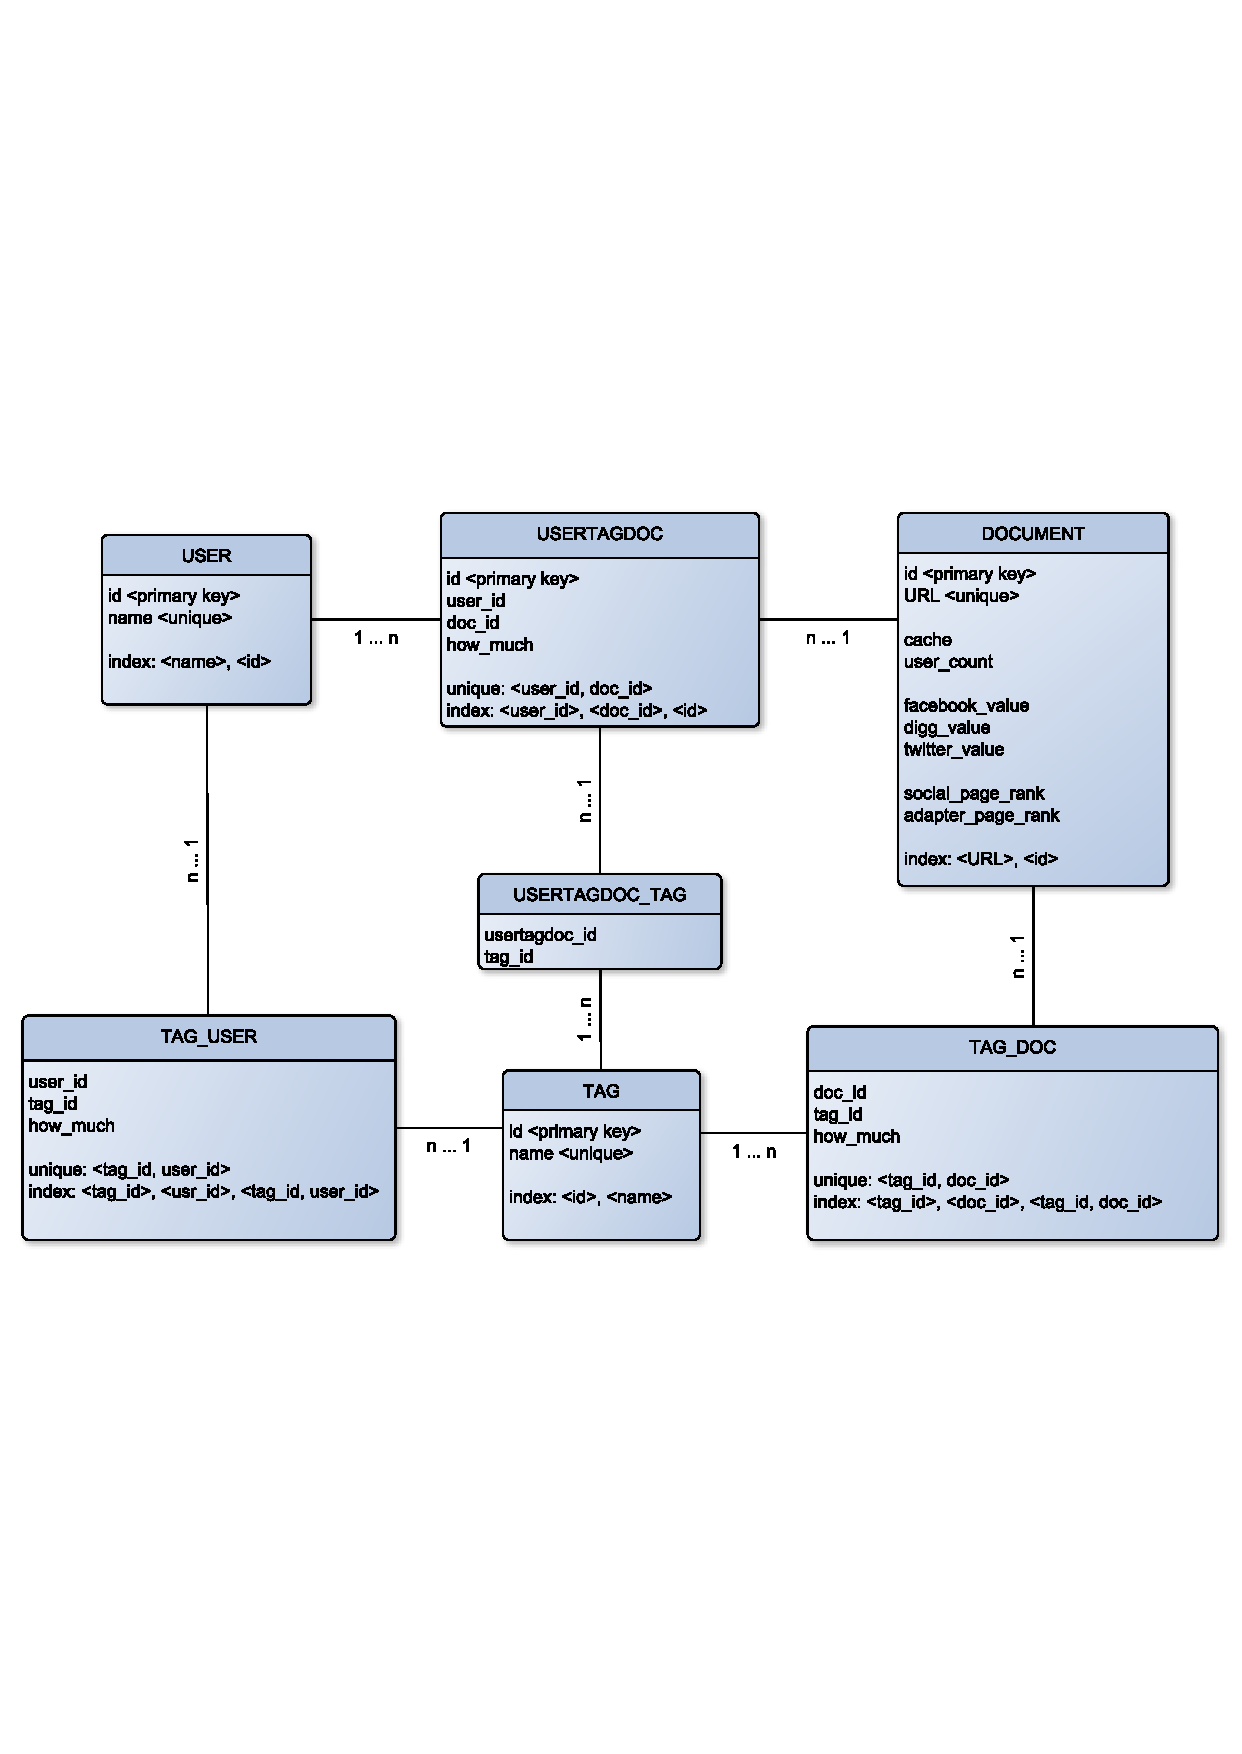
\includegraphics[  trim = 3mm 87mm 4mm 87mm, clip = true, width=\textwidth]{database.pdf}
\caption{Schemat bazy danych}
\label{fig:db_fig}
\end{figure}

Baza danych składa się z trzech głównych tabel: USER, DOCUMENT i TAG. Zawierają one informację na temat, odpowiednio, użytkowników, dokumentów i adnotacji pobrane z serwisu delicous. W bazie danych znajdują się też tabele: USERTAGDOC i USERTAGDOC\_TAG, które służą do zapisania relacji między użytkownikami a dokumentami (USERTAGDOC) i adnotacjami ich opisującymi (USERTAGDOC\_TAG). W tych tabelach zapisane są  informacje na temat tego czy dany użytkownik dodał dokument do serwisu i jakimi tagami została dana strona opisana.

\subsection{Pomocnicze tabele i pola. Indeksy}
Dodatkowo w bazie danych (rys \ref{fig:db_fig} )znajdują się dwie tabele: TAG\_DOC i TAG\_USR. W tabelach tych zapisywane są dane wyliczone z pozostałych tabel. W tabeli TAG\_DOC znajdują się informację na temat tego ilu użytkowników dodało dany dokument $doc_i$  i opisało go tagiem $tag_k$. Odpowiednia w tabeli TAG\_USR znajdują się informację na temat ilości różnych dokumentów dodanych przez użytkownika $usr_n$ i opisanych tagiem $tag_m$. Dane ilości różnych tagów którymi użytkownik $usr_l$ opisał dokument $doc_j$ przechowywane są w już istniejącej tabeli USERTAGDOC. 

Tabele TAG\_DOC, TAG\_USR i pole how\_much w tabeli USERTAGDOC zostają wypełnione w czasie preprocessingu. Dane te posłużą  później do utworzenia macierzy, używanych przez algorytmy Social PageRank i Adapted PageRank. 


W tabelach na różnych polach zostały dodane indeksy. Przyśpieszają one działanie aplikacji, pozwalają na szybsze operacja przy często używanych polach. Główne indeksy zostały zaznaczone na rysunku \ref{fig:db_fig}

\subsection{Listing}
Poniżej znajduje się listing zapytania SQL tworzącego tabele w bazie danych.

\lstset{language=SQL}  
\begin{lstlisting}[frame=lines, caption={Skrypt tworzący tabele w bazie danych}, label={sql_all}] ]


CREATE TABLE `DOCUMENT` (
 `id` bigint(20) NOT NULL AUTO_INCREMENT,
 `url` varchar(255) NOT NULL,
 `digg_value` int(11) DEFAULT '0',
 `facebook_value` int(11) DEFAULT '0',
 `twitter_value` int(11) DEFAULT '0',
 `page_fetch` tinyint(1) DEFAULT '0',
 `tag_count` bigint(20) DEFAULT NULL,
 `user_count` bigint(20) DEFAULT NULL,
 `cache` text,
 `adapted_page_rank` double DEFAULT NULL,
 `social_page_rank` double DEFAULT NULL,
 PRIMARY KEY (`id`),
 UNIQUE KEY `url` (`url`)
) 

CREATE TABLE `TAG` (
 `id` bigint(20) NOT NULL AUTO_INCREMENT,
 `doc_count` bigint(20) DEFAULT NULL,
 `doc_dist_count` bigint(20) DEFAULT NULL,
 `tag` varchar(255) NOT NULL,
 `user_count` bigint(20) DEFAULT NULL,
 `adapted_page_rank` double DEFAULT NULL,
 PRIMARY KEY (`id`),
 UNIQUE KEY `tag` (`tag`)
)

CREATE TABLE `TAG_DOC` (
 `id` bigint(20) NOT NULL AUTO_INCREMENT,
 `doc_id` bigint(20) DEFAULT NULL,
 `tag_id` bigint(20) DEFAULT NULL,
 `how_much` int(11) DEFAULT '1',
 PRIMARY KEY (`id`),
 UNIQUE KEY `tag_doc` (`doc_id`,`tag_id`),
 KEY `doc_id` (`doc_id`,`tag_id`),
 KEY `tag_doc_doc` (`doc_id`),
 KEY `tag_doc_tag` (`tag_id`)
) 

CREATE TABLE `TAG_USR` (
 `id` bigint(20) NOT NULL AUTO_INCREMENT,
 `user_id` bigint(20) DEFAULT NULL,
 `tag_id` bigint(20) DEFAULT NULL,
 `how_much` int(11) DEFAULT '1',
 PRIMARY KEY (`id`),
 UNIQUE KEY `tag_user` (`user_id`,`tag_id`),
 KEY `user_id` (`user_id`,`tag_id`),
 KEY `tag_usr_doc` (`tag_id`),
 KEY `tag_usr_usr` (`user_id`)
)

CREATE TABLE `USER` (
 `id` bigint(20) NOT NULL AUTO_INCREMENT,
 `doc_count` bigint(20) DEFAULT NULL,
 `name` varchar(255) DEFAULT NULL,
 `new_data` tinyint(1) DEFAULT '1',
 `tag_count` bigint(20) DEFAULT NULL,
 `tag_dist_count` bigint(20) DEFAULT NULL,
 `adapted_page_rank` double DEFAULT NULL,
 PRIMARY KEY (`id`),
 UNIQUE KEY `name` (`name`)
)


CREATE TABLE `USERTAGDOC` (
 `id` bigint(20) NOT NULL AUTO_INCREMENT,
 `doc_id` bigint(20) DEFAULT NULL,
 `user_id` bigint(20) DEFAULT NULL,
 `how_much` int(11) DEFAULT NULL,
 PRIMARY KEY (`id`),
 UNIQUE KEY `user_id` (`user_id`,`doc_id`),
 KEY `FKB30EFAE96714BC07` (`doc_id`),
 KEY `FKB30EFAE9520DD4E4` (`user_id`),
 CONSTRAINT `FKB30EFAE9520DD4E4` FOREIGN KEY (`user_id`) REFERENCES
`user` (`id`),
 CONSTRAINT `FKB30EFAE96714BC07` FOREIGN KEY (`doc_id`) REFERENCES
`document` (`id`)
) 


CREATE TABLE `USERTAGDOC_TAG` (
 `USERTAGDOC_id` bigint(20) NOT NULL,
 `tags_id` bigint(20) NOT NULL,
 KEY `FK4C01D124CA702D03` (`tags_id`),
 KEY `FK4C01D1243D83CB28` (`USERTAGDOC_id`),
 CONSTRAINT `FK4C01D1243D83CB28` FOREIGN KEY (`USERTAGDOC_id`)
REFERENCES `usertagdoc` (`id`),
 CONSTRAINT `FK4C01D124CA702D03` FOREIGN KEY (`tags_id`) REFERENCES
`tag` (`id`)
) 

\end{lstlisting}

